\graphicspath{ {mainmatter/Wang_2004/} }

\title*{2004: On-the-fly Programming: Using Code as an Expressive Musical Instrument}
\titlerunning{Code as an Expressive Musical Instrument}

\author{Ge Wang and Perry R. Cook}
\authorrunning{Wang and Cook}

%\institute{Ge Wang \at Center for Computer Research in Music and Acoustics (CCRMA), Stanford University, \email{gewang@cs.princeton.edu}
%\and Perry R. Cook \at Department of Computer Science (also Music) (Emeritus), Princeton University, \email{prc@cs.princeton.edu}}
%
%
\maketitle

\abstract*{On-the-fly programming is a style of programming in which the programmer/performer/composer augments and modifies the program while it is running, without stopping or restarting, in order to assert expressive, programmable control at runtime.   Because of the fundamental powers of programming languages, we believe the technical and aesthetic aspects of on-the-fly programming are worth exploring. In this paper, we present a formalized framework for on-the-fly programming, based on the ChucK synthesis language, which supports a truly concurrent audio programming model with sample-synchronous timing, and a highly on-the-fly style of programming.  We first provide a well-defined notion of on-the-fly programming.  We then address four fundamental issues that confront the on-the-fly programmer: timing, modularity, conciseness, and flexibility. Using the features and properties of ChucK, we show how it solves many of these issues.  In this new model, we show that (1) concurrency provides natural modularity for on-the-fly programming, (2) the timing mechanism in ChucK guarantees on-the-fly precision and consistency, (3) the Chuck syntax improves conciseness, and (4) the overall system is a useful framework for exploring on-the-fly programming.  Finally, we discuss the aesthetics of on-the-fly performance.}


\section{Introduction}

Due to their fundamental expressive power, programming languages and systems
play a pivotal role in the composition, performance, and experimentation of
computer audio and electro-acoustic music.  For the most part, however, the
design and writing of computer music programs have been limited to off-line
development and preparation, leaving only the finished program to ``go live.'' 
Thus, the gamut of runtime possibility is prescribed by the predetermined
functionalities, programmed ahead of time.

An \textit{on-the-fly programmable system} provides the ability to write/modify,
compile, execute new/existing code, and then integrate it into a program while it
is running, with precise timing and synchronization.  The goal of on-the-fly
programming is to enable programmers/performers/composers to actively modify
their programs on-line without having to stop, code, and restart.  For example,
performers could add/change modules in their synthesis or composition programs,
or modify mappings to their controllers during a live performance.  Similarly,
composers can experiment with their programs on-line, modifying synthesis
components, shaping or perfecting a sound, or changing compositional elements,
without having to restart.

\begin{figure}[t]
\centering
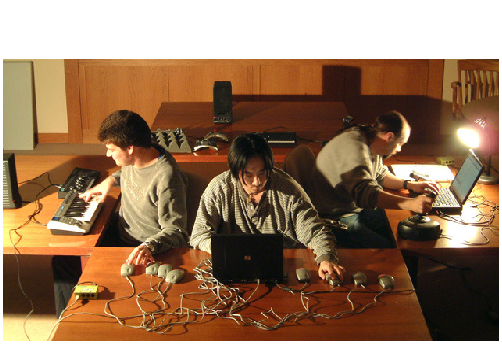
\includegraphics[width=\textwidth]{img-1-eps-converted-to-crop.pdf}
\caption{On-the-fly programmers in session.}
\label{Wang:img-1}
\end{figure}

The features of the programming tool inevitably shape both the means by which tasks are implemented as well as the end product.  By bringing the power and expressiveness of the programming language into runtime, an on-the-fly programming system has the potential to fundamentally enhance the interaction between the performer/composer and the systems they create and control. \textit{Code becomes a real-time, expressive instrument}.  We believe such a potential is worth exploring.

In this work, we define on-the-fly programming and provide a formal programming model based on ChucK\footnote{\url{http://chuck.cs.princeton.edu/}} \cite{Wang:2015}, leveraging its properties of timing and concurrency. In addition, we discuss an open on-the-fly programming aesthetic.  To this end, Section 2 defines on-the-fly programming and identifies some of the central issues that an on-the-fly programming system should address, and also discusses on-the-fly elements found in existing programming languages. Section 3 provides an overview of the features and properties of ChucK that are relevant to on-the-fly programming.  Based on these features and properties, Section 4 defines a formal framework and programming model for on-the-fly programming.  We show how the properties of ChucK are preserved and extended in the new model. Section 5 uses the on-the-fly model and discusses an aesthetic for live performance.  Finally, we conclude and discuss future work in Section 6.


\section{Background}

Elements of on-the-fly programming have existed in computer music systems and languages in various forms.  Some performers have incorporated various runtime programmable aspects in their systems and methodologies.  However, there has not been a formalized framework or a genuinely on-the-fly system that defines and addresses all the issues of runtime programmability.

\subsection{Definition}

In order to discuss the technical and aesthetic aspects of on-the-fly programming, we first provide a well-defined notion of what it is.  In the context of this study, we define on-the-fly programming to consist of all the following elements:

\begin{itemize}
	\item First executing an existing program, or possibly an empty program---we will call this P.
	\item Subsequently writing new code segment Q in a programming language, and adding it (possibly with type-checking and compilation) to the existing program P, forming program P.'  Specifically, by ``adding Q to P,'' we mean (1) Q now runs in the address space of P, potentially sharing data, and (2) there is a strong notion of temporal correspondence between Q and P, such that Q can access the timing of P and also synchronized with P.  We shall see an example of this in \textit{Section 4}.
	\item Modifying parts of the program P while it is executing.  This is general enough to include anything that modifies the program structure or logic.  We intentionally leave this open, for each system may have its own way of modifying the program.  We will see that in ChucK, the program can be modified via replacement of concurrent, modular code blocks using the internal timing and virtual machine interface.
\end{itemize}

\subsection{Challenges}

In order to bring the power and general expressiveness of programming languages
into on-the-fly programming, several fundamental challenges must be addressed. 
We have identified the following issues:

\begin{description}[Type 1]
	\item[Modularity:]{code sections must be modular so the programmer can reason about them or modify them independently.  Furthermore, the augmented code must work together in the same address space and namespace.}
	\item[Timing:]{there must be a strong consistency and notion of time and timing between the existing and new parts of the program.  Sequential on-the-fly code segments need to start and stop with precision.}
	\item[Conciseness and manageability:]{given the substantial time constraints, we ask: how can ideas be expressed concisely in code?   How do we reason about time and data flow easily?}
	\item[Flexibility:]{how flexible is the system?  Does it allow programmers to take advantage of the expressive power of programming languages in a real-time setting?}
\end{description}

Taking these challenges into account, and using the definition provided, we next evaluate some existing languages and systems.  In Sections 3 and 4, we will show how features of ChucK provide a solution to each of these challenges.

\subsection{Existing Languages and Systems}

Ever since Music I \cite{Lyon:2002}, there has since been many computer music programming
languages and systems. \cite{Cook:1999a,Dannenberg:1997,Loy:1985,Lyon:2002,Pope:1993}  Many of these, especially the earlier
ones were designed to operate in a non-real-time manner.  They are interesting
and influential to more modern languages, but are not directly relevant to this
study of on-the-fly programming.  Additionally, performers have used runtime
programmable elements during live performance and/or rehearsal. Examples go back
as far as Jim Horton, Tim Perkis, and John Bischoff of The League of Automatic
Composers, who tweaked live electronics with microcomputers (KIM's) during
performance, and George Lewis, as well as the network group The Hub, who used
languages like FORTH to modify their systems online, to more recent laptop
computer musicians who construct and use various on-the-fly tools, including
command-line, shell scripts, and homemade software tools \cite{Collins:2003}.

Of the real-time computer music languages, on-the-fly programming elements can
be found in Max \cite{Puckette:1991} and Pure Data \cite{Puckette:1996}, which allow programmers to alter parts
of their patch while it is running.  However, \textit{data-flow} (unit generators
and patches) is easy to represent whereas \textit{timing}, in general, is
significantly more difficult to discern and manipulate.  Also, there are no
mechanisms for programming smooth transitions when connecting sub-patches. 
Finally, the programming semantic can prove to be rigid when trying to
incrementally add new logic to existing patches and modules.

SuperCollider \cite{McCartney:2002}, with its client/server architecture allows for synthesis
patches to be compiled/interpreted on the client and sent to the server, where
they can form a network of language-neutral synthesis elements, on-the-fly. 
However, there lacks a formal language-level framework (in addition to parameters
to unit generators) for describing timing across all parts of the program as well
as for exerting low-level timing control.

\section{Chuck Overview}

ChucK is designed to be a concurrent, on-the-fly audio programming language
 \cite{Wang:2003}.  It is not based on a single existing language but built from the ground
up.  It is \textit{strongly-typed} and \textit{strongly-timed}, and runs over a
virtual machine with a native audio engine and a user-level scheduler.  Several
features of ChucK directly support/encourage on-the-fly programming:

\begin{itemize}
	\item A straightforward way to connect \textit{data-flow }/ unit generators.
	\item A sample-synchronous timing mechanism that provides a consistent and unified
view of time.  Timing is embedded directly in the program flow, making ChucK
programs easy to maintain and reason about.  \textit{Data-flow }is fundamentally
decoupled from\textit{ time}.
	\item A cooperative multi-tasking, concurrent programming model \textit{based on time}
that allows programmers to add concurrency easily and scalably.  Synchronization
is accurately and automatically derived from the timing mechanism.
	\item Multiple, simultaneous, arbitrary, and dynamically programmable control rates
via the timing mechanism and concurrency.
	\item A compiler and virtual machine that run in the same process, both accessible
from within the language.
\end{itemize}

As a result, ChucK provides a programming model that addresses several areas in
computer music programming: representation, level of control of data-flow and
time, and concurrency.  We summarize the features and properties of ChucK in the
context of these areas.  In doing so, we lay the foundation for describing the
semantics of the on-the-fly programming model in \textit{Section 4}.

\subsection{Representation}

Representation deals with the elegant mapping of audio concepts to syntactical
and semantic constructs in the language.  An effective representation should also
be straightforward to reason about and maintain.  ChucK addresses this problem in
both its syntax and semantics.  The syntax provides a means to specify
\textit{data-flow;} the timing semantics specify when computations occur.  In
this way, both high-level manipulation and low-level control is achieved.  We
discuss the syntactical portion here, and reserve the discussion about timing
semantics for \textit{Section 3.2}.

At the heart of the syntax is the \textit{ChucK operator}: a group of related
operators (\texttt{=>}, \texttt{+=>}) that denote interconnection
and direction of data flow.  A unit generator (\textit{ugen}) patch can be
quickly and clearly constructed by using \texttt{=>} to connect
\textit{ugen}'s in a strongly ordered, left-to-right manner (Figure~\ref{Wang:img-2}).  By
default,  \texttt{\texttt{=>}} \textit{only} deals with
\textit{data-flow}, leaving the issues of \textit{time }to the timing mechanism. 
Parameters to the unit generators can also be modified using the ChucK operator.


\begin{figure}[t]
\centering
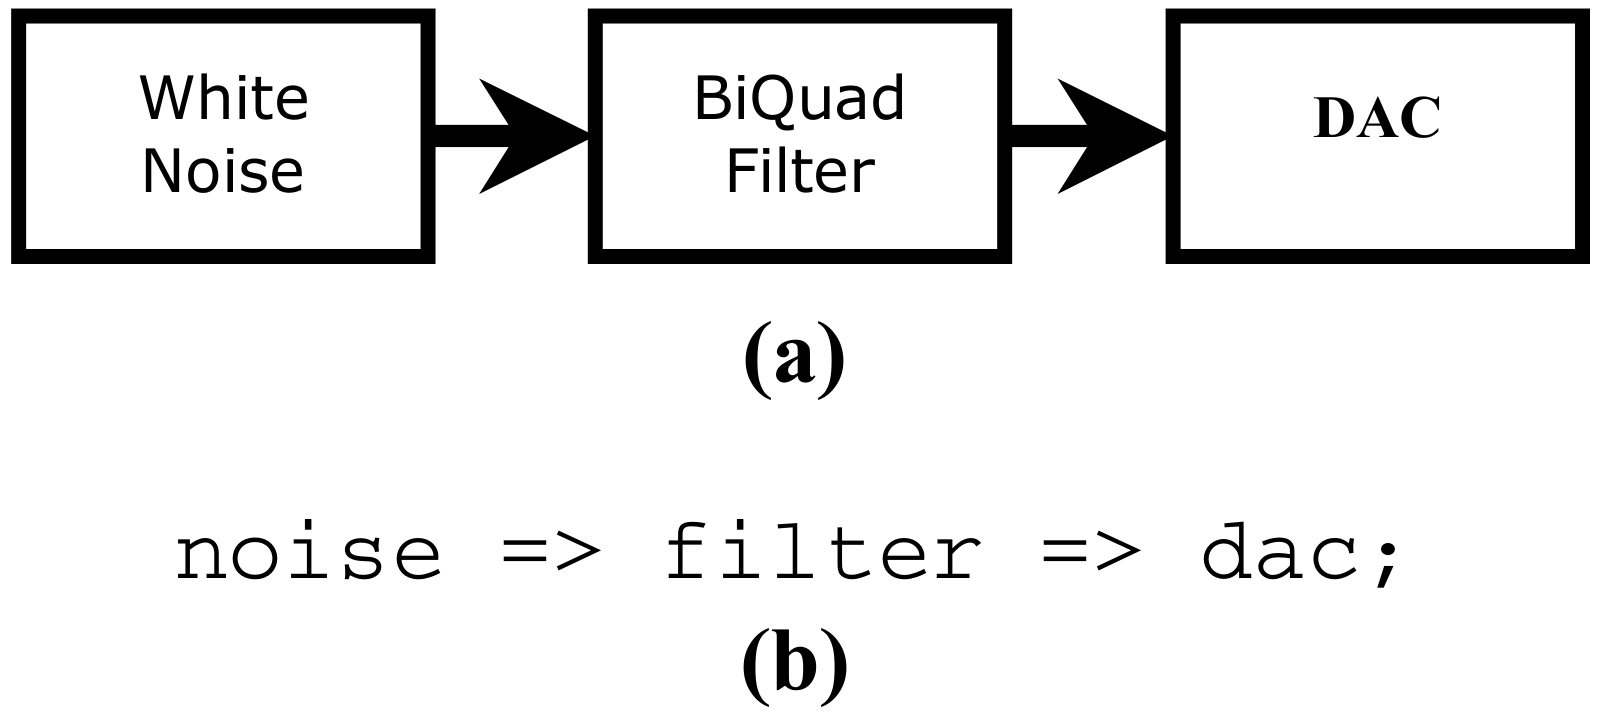
\includegraphics[width=60mm]{fig2.png}
\caption{(a) A noise-filter patch using three unit generators. (b) ChucK statement representing the patch.  \textit{dac} is the global sound output variable.}
\label{Wang:img-2}
\end{figure}


\subsection{Level of Control}

The level of control and abstraction provided by the language shapes what can be done with the language and how it is used.  In the context of audio programming, we are concerned not only with control over \textit{data} but also over \textit{time}.  The latter deals with control rates and the manner in which time is manipulated and reasoned about in the language.  Thus, the question is: \textit{what is the appropriate level and granularity of control for data and time?}

The solution in ChucK is to provide many levels and granularity of control over data and time.  The key to having a flexible level of control lies in the ChucK timing mechanism, which consists of two parts.  First, time (\verb!time!) and duration (\verb!dur!) are native types in the language. Time refers in a point in time whereas duration is a finite amount of time. Basic duration values are provided by default: \verb!samp! (the duration between successive samples), \verb!ms! (millisecond), \verb!second!, \verb!minute!, \verb!hour!, \verb!day!, and \verb!week!.  Additional durations can be inductively constructed using arithmetic operations on existing time and duration values.

Secondly, there is a special keyword \verb!now! (of type \verb!time!) that holds the current ChucK time, which starts from 0 (at the beginning of the program execution).  \verb!now! is the key to reasoning about and manipulating time in ChucK.  Programs can read the globally consistent ChucK time by reading the value of \verb!now!.  Also, by assigning time values or adding duration values to \verb!now! causes time to \textit{advance}.  As an important \textit{side effect}, this operation causes the current process to \textit{block} (allowing audio to compute) until \verb!now! actually reaches the desired point in time (Figure~\ref{Wang:img-3}).  We call this \textit{synchronization to time}.

% Tried to add code, but more consistent to use images for each of them, since it was like that in the original.
%
% \begin{verbatim}
% // construct a unit generator patch
% noise => biquad => dac;
% // loop: update biquad every 100 ms
% while( true )
% {
%     // sweep biquad center frequency 
%     500 + 300 * sin(now*FC) => biquad.freq;
%     // advance time by 100 ms
%     100::ms +=> now;
% }
% \end{verbatim}

\begin{figure}[t]
\centering
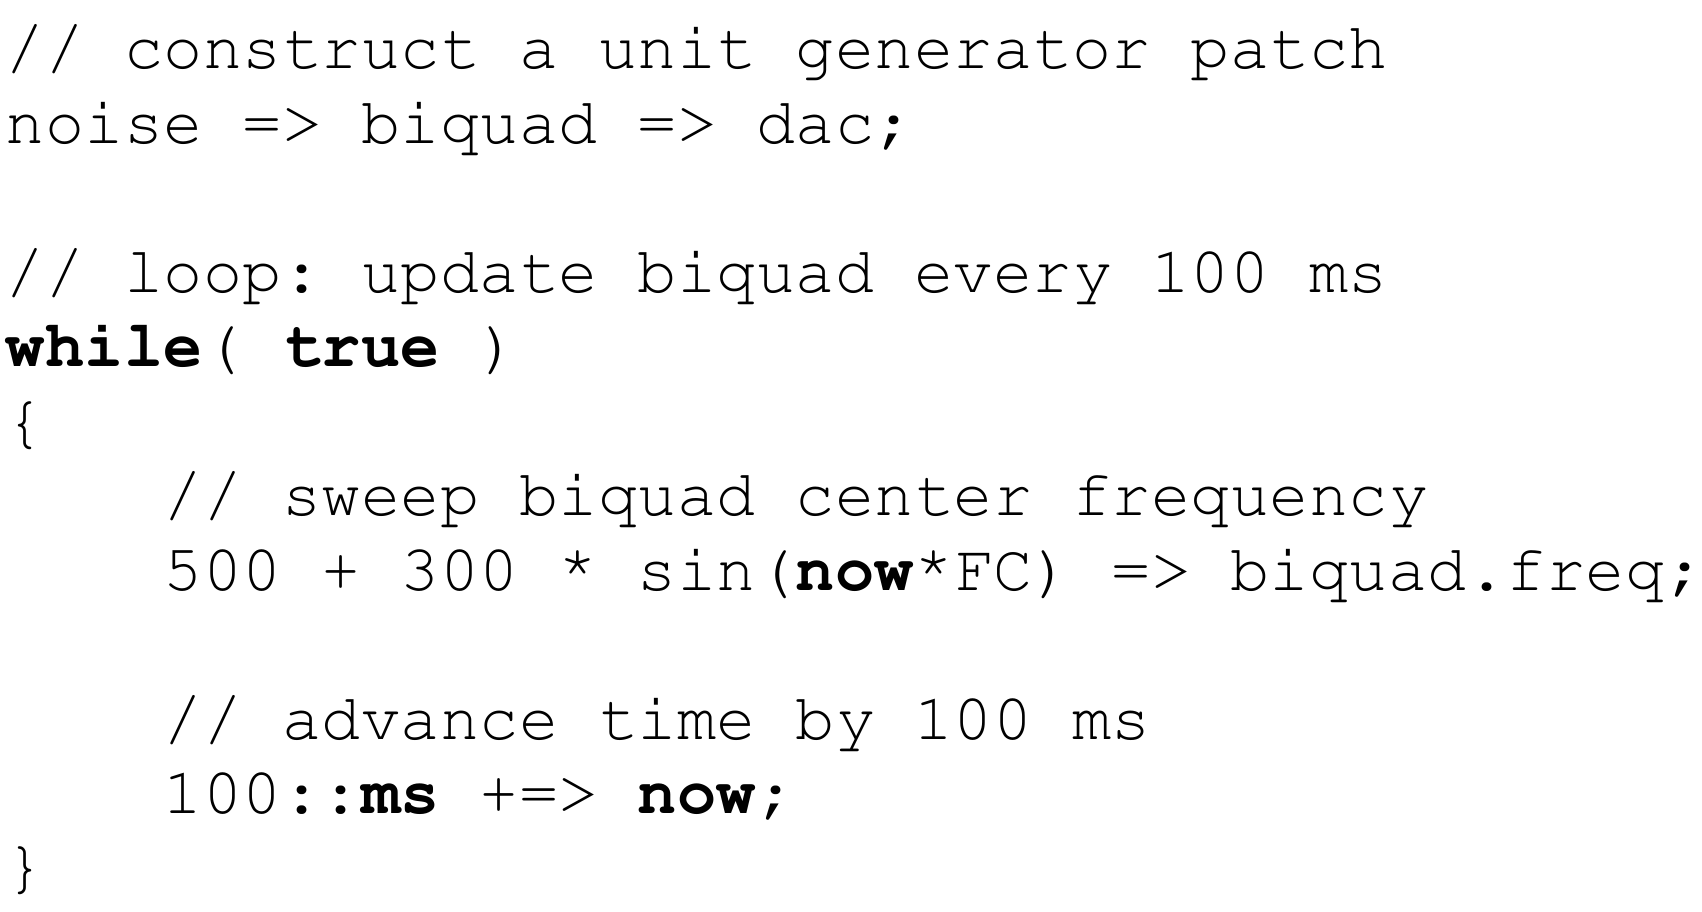
\includegraphics[width=70mm]{fig3.png}
\caption{\textit{A control loop}.  The $!=>!$ ChucK operator is used to change biquad's frequency control parameter.  The last line of the loop causes time to \textit{advance} by 100 milliseconds---this can be thought of as the control rate.}
\label{Wang:img-3}
\end{figure}




This mechanism provides a consistent, sample-synchronous view of time and embeds
timing control directly in the code.  This strong correspondence between timing
and code makes programs easier to write and maintain.  \textit{Data-flow} is
decoupled from\textit{ time}.  Furthermore, the timing mechanism allows for the
control rate to be fully throttled by the programmer---audio rates, control
rates, and high-level musical timing are unified under the same timing mechanism.

\subsection{Concurrent Audio Programming}

Sound and music are often the simultaneity of many precisely timed entities and
events.  There have been many ways devised to represent simultaneity \cite{Dannenberg:1997,Loy:1985,Pope:1993} in
computer music languages.  ChucK uniquely presents a concurrent and precisely
timed programming model for audio.  This aspect of the language is a powerful
extension of the timing mechanism and is essential to our model of on-the-fly
programming.

The intuitive goal of concurrent audio programming is straightforward: to write
concurrent code that shares data as well as time (Figure~\ref{Wang:img-4}).



\begin{figure}[t]
\centering
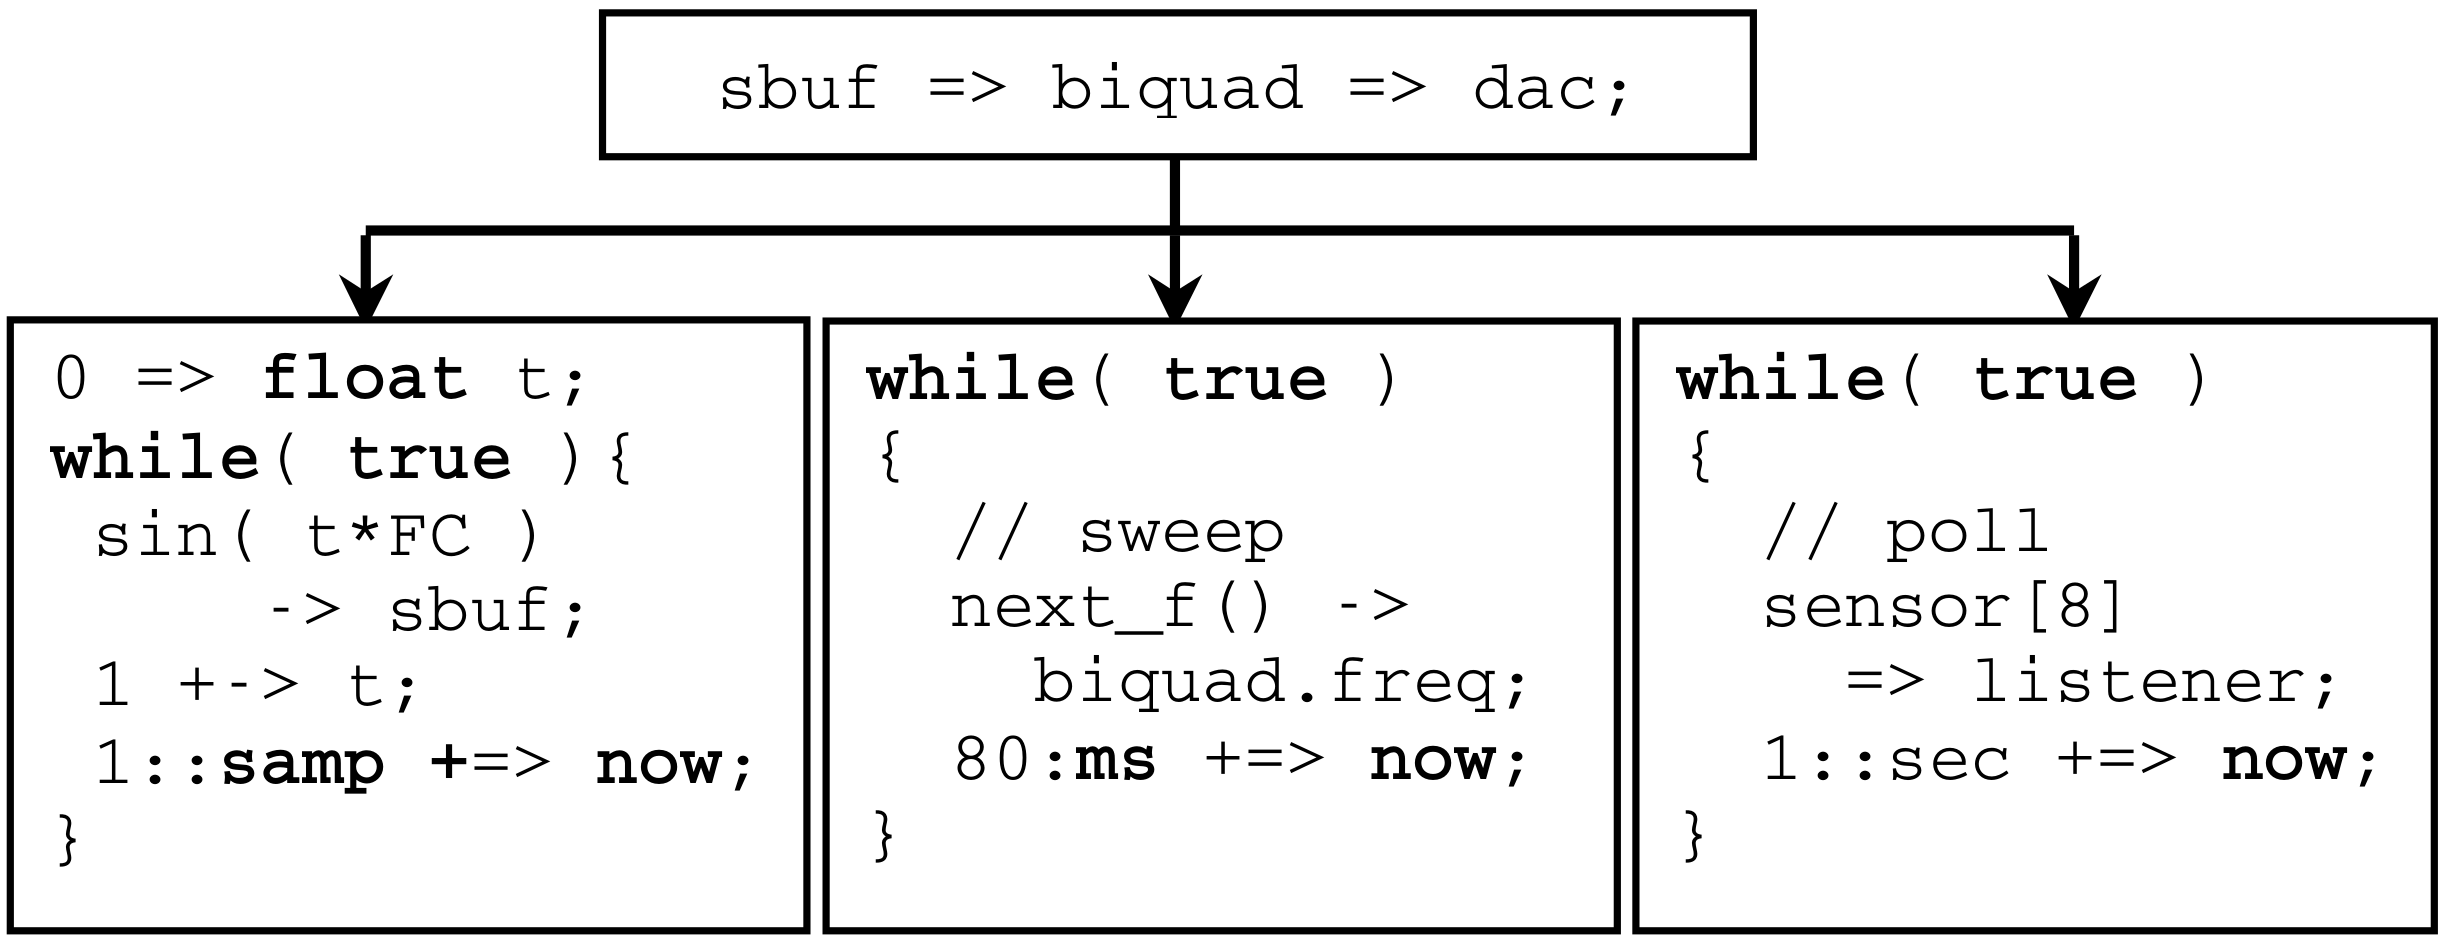
\includegraphics[width=90mm]{fig4.png}
\caption{A unit generator patch and three concurrent paths of execution at different control rates.}
\label{Wang:img-4}
\end{figure}



ChucK introduced the concepts of \textit{shreds} and the \textit{shreduler}.  A
shred is a concurrent entity like a thread \cite{Birrell:1989}.  But unlike threads, a shred is a
deterministic shred of computation, synchronized by time.  Each of the concurrent
paths of execution in Figure~\ref{Wang:img-4} can be realized by a shred.  They can reside in
separate source files or be dynamically spawned (\textit{sporked}) from a single
parent shred.

The key insight to understanding concurrency in ChucK is that \textit{shreds are
automatically synchronized by time}. Two independent shreds can execute with
precise timing relative to each other and the virtual machine, without any
knowledge of each other.  This is a powerful mechanism for specifying and
reasoning about time locally and globally in a synthesis program.  Furthermore,
it allows for any number of different control rates to execute concurrently and
accurately.  ChucK concurrency is orthogonal in that programmers can add
concurrency without modification to existing code.  It is also scalable, because
shreds are implemented as efficient user-level constructs in the ChucK Virtual
Machine.  Indeed, this mechanism is used in \textit{Section 4} to synchronize
on-the-fly program modules.

\subsection{ChucK Virtual Machine}

ChucK code is compiled and executed in the ChucK Virtual Machine, which consists
of an on-the-fly compiler, a virtual instruction interpreter, a native audio
engine, the \textit{shreduler}, and a I/O manager (Figure~\ref{Wang:img-5}).  The on-the-fly
compiler, the \textit{shreduler}, and the virtual machine itself can be accessed
as global objects from within the language.  For example, a shred can request the
compiler to parse and type-check a piece of code dynamically, and then
\textit{shredule} the code to execute as part of the same process.  This
mechanism, along with the timing and concurrency form the foundation for our
on-the-fly programming model.


\begin{figure}[t]
\centering
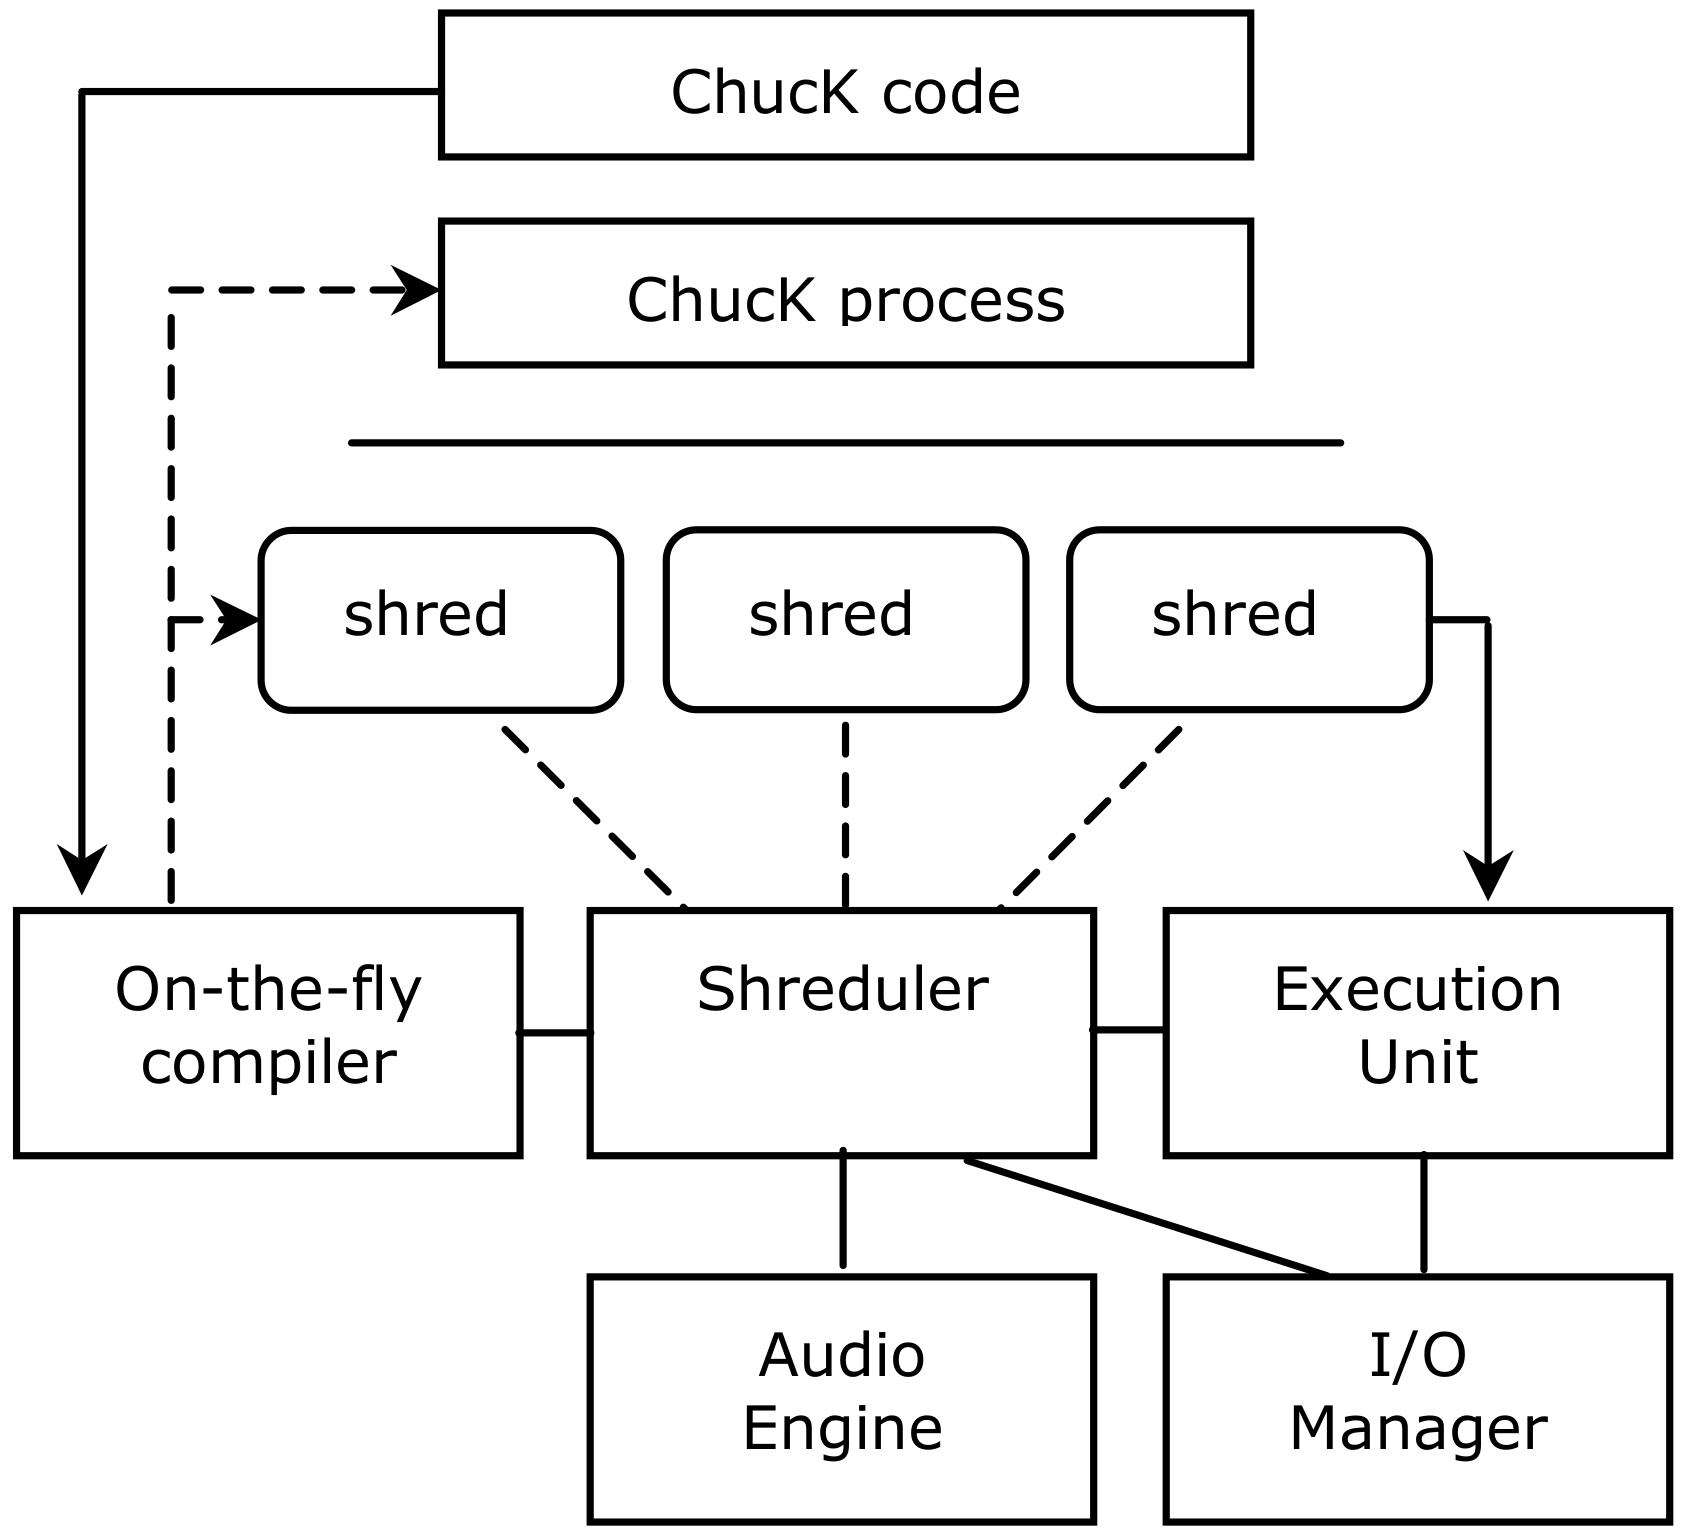
\includegraphics[width=70mm]{fig5.png}
\caption{The ChucK Virtual Machine runtime.}
\label{Wang:img-5}
\end{figure}



\section{The On-the-fly Model}

In this section, we describe a formal on-the-fly programming model, based on the
features of ChucK.  We do so in two parts: \textit{external} and
\textit{internal} semantic.  We reason about key properties in the model and
present an example.  We show that just as concurrency in ChucK is a natural
extension of the timing mechanism, we can leverage the timing mechanism and
concurrency to address the challenges of on-the-fly programming.

\subsection{Operational Semantics}

\subsubsection{External Interface}

The on-the-fly programming model, at the high-level, can be described in the
following way.  A ChucK virtual machine begins execution, generating samples (as
necessary), keeping time, and waiting for incoming shreds.  ChucK shreds can be
\textit{assimilated} on-the-fly into the virtual machine, sharing the memory
address space and global timing mechanism, and is said to be \textit{active}. 
Similarly, an active shred can be \textit{dissimilated}, or removed from the
virtual machine, or it can be suspended or be replaced by another shred.  This
interface is designed to be simple, and delegates the actual timing and
synchronization logic to the code within the shred (discussed in \textit{Section
4.1.2}), leaving this flexibility to the programmer.

The high level commands to the external interface are listed below.  They can be
invoked on the command line, in ChucK programs (as functions calls to the {\small
machine} and {\small compiler} objects), over the network, via customized
graphical interfaces, or by other appropriate means.

\begin{description}[Type 1]
	\item[Execute]{begins a new instance of the virtual machine in a new
address space.  Typically, this operation is used at the beginning of the
session.  Multiple instances of the virtual machine can coexist.  The
\textit{shreduler} begins to keep track of time.}
	\item[Add]{type-checks and compiles a new shred (from a ChucK source file,
a string containing ChucK code, or a pre-compiled shred).  If there are no
compilation errors, the shred is allocated and \textit{sporked} in the virtual
machine with a unique ID.  A new virtual stack is allocated, and the shred is
\textit{shreduled} immediately to execute from the beginning.  When add fails due
to compilation errors, the virtual machine continues to run as before while the
programmer can attempt to debug, correct, and add the code.}
	\item[Remove]{removes a shred by ID or name from the virtual machine.  The
shred's exit point function (if defined) is invoked and the shred and relevant
child objects are garbage collected.}
	\item[Suspend]{similar to remove, except the shred's suspend() function (if
defined) is invoked, and the shred is removed by the \textit{shreduler} and
placed on the suspended list.}
	\item[Resume]{resumes a suspended shred, calls its resume() function and
places it in the \textit{shreduler}'s ready-to-run list.  The shred will resume
execution at the suspended point in the code.}
	\item[Replace]{invokes a remove operation followed by an add.  An option
exists for making the operation \textit{atomic}.}
	\item[Status]{queries the status of the virtual machine for the following
types of information: (1) a list of active/suspended shreds ID's,
source/filename, duration since assimilation (\textit{spork} time), and (2)
information on virtual machine state: currently executing shred,
\textit{shreduler} timeline, and CPU / VM usage by various parts of the system.}
\end{description}

For example, Figure~\ref{Wang:img-6} shows code that adds, replaces, and removes two shreds
using separate methods.

\begin{figure}[t]
\centering
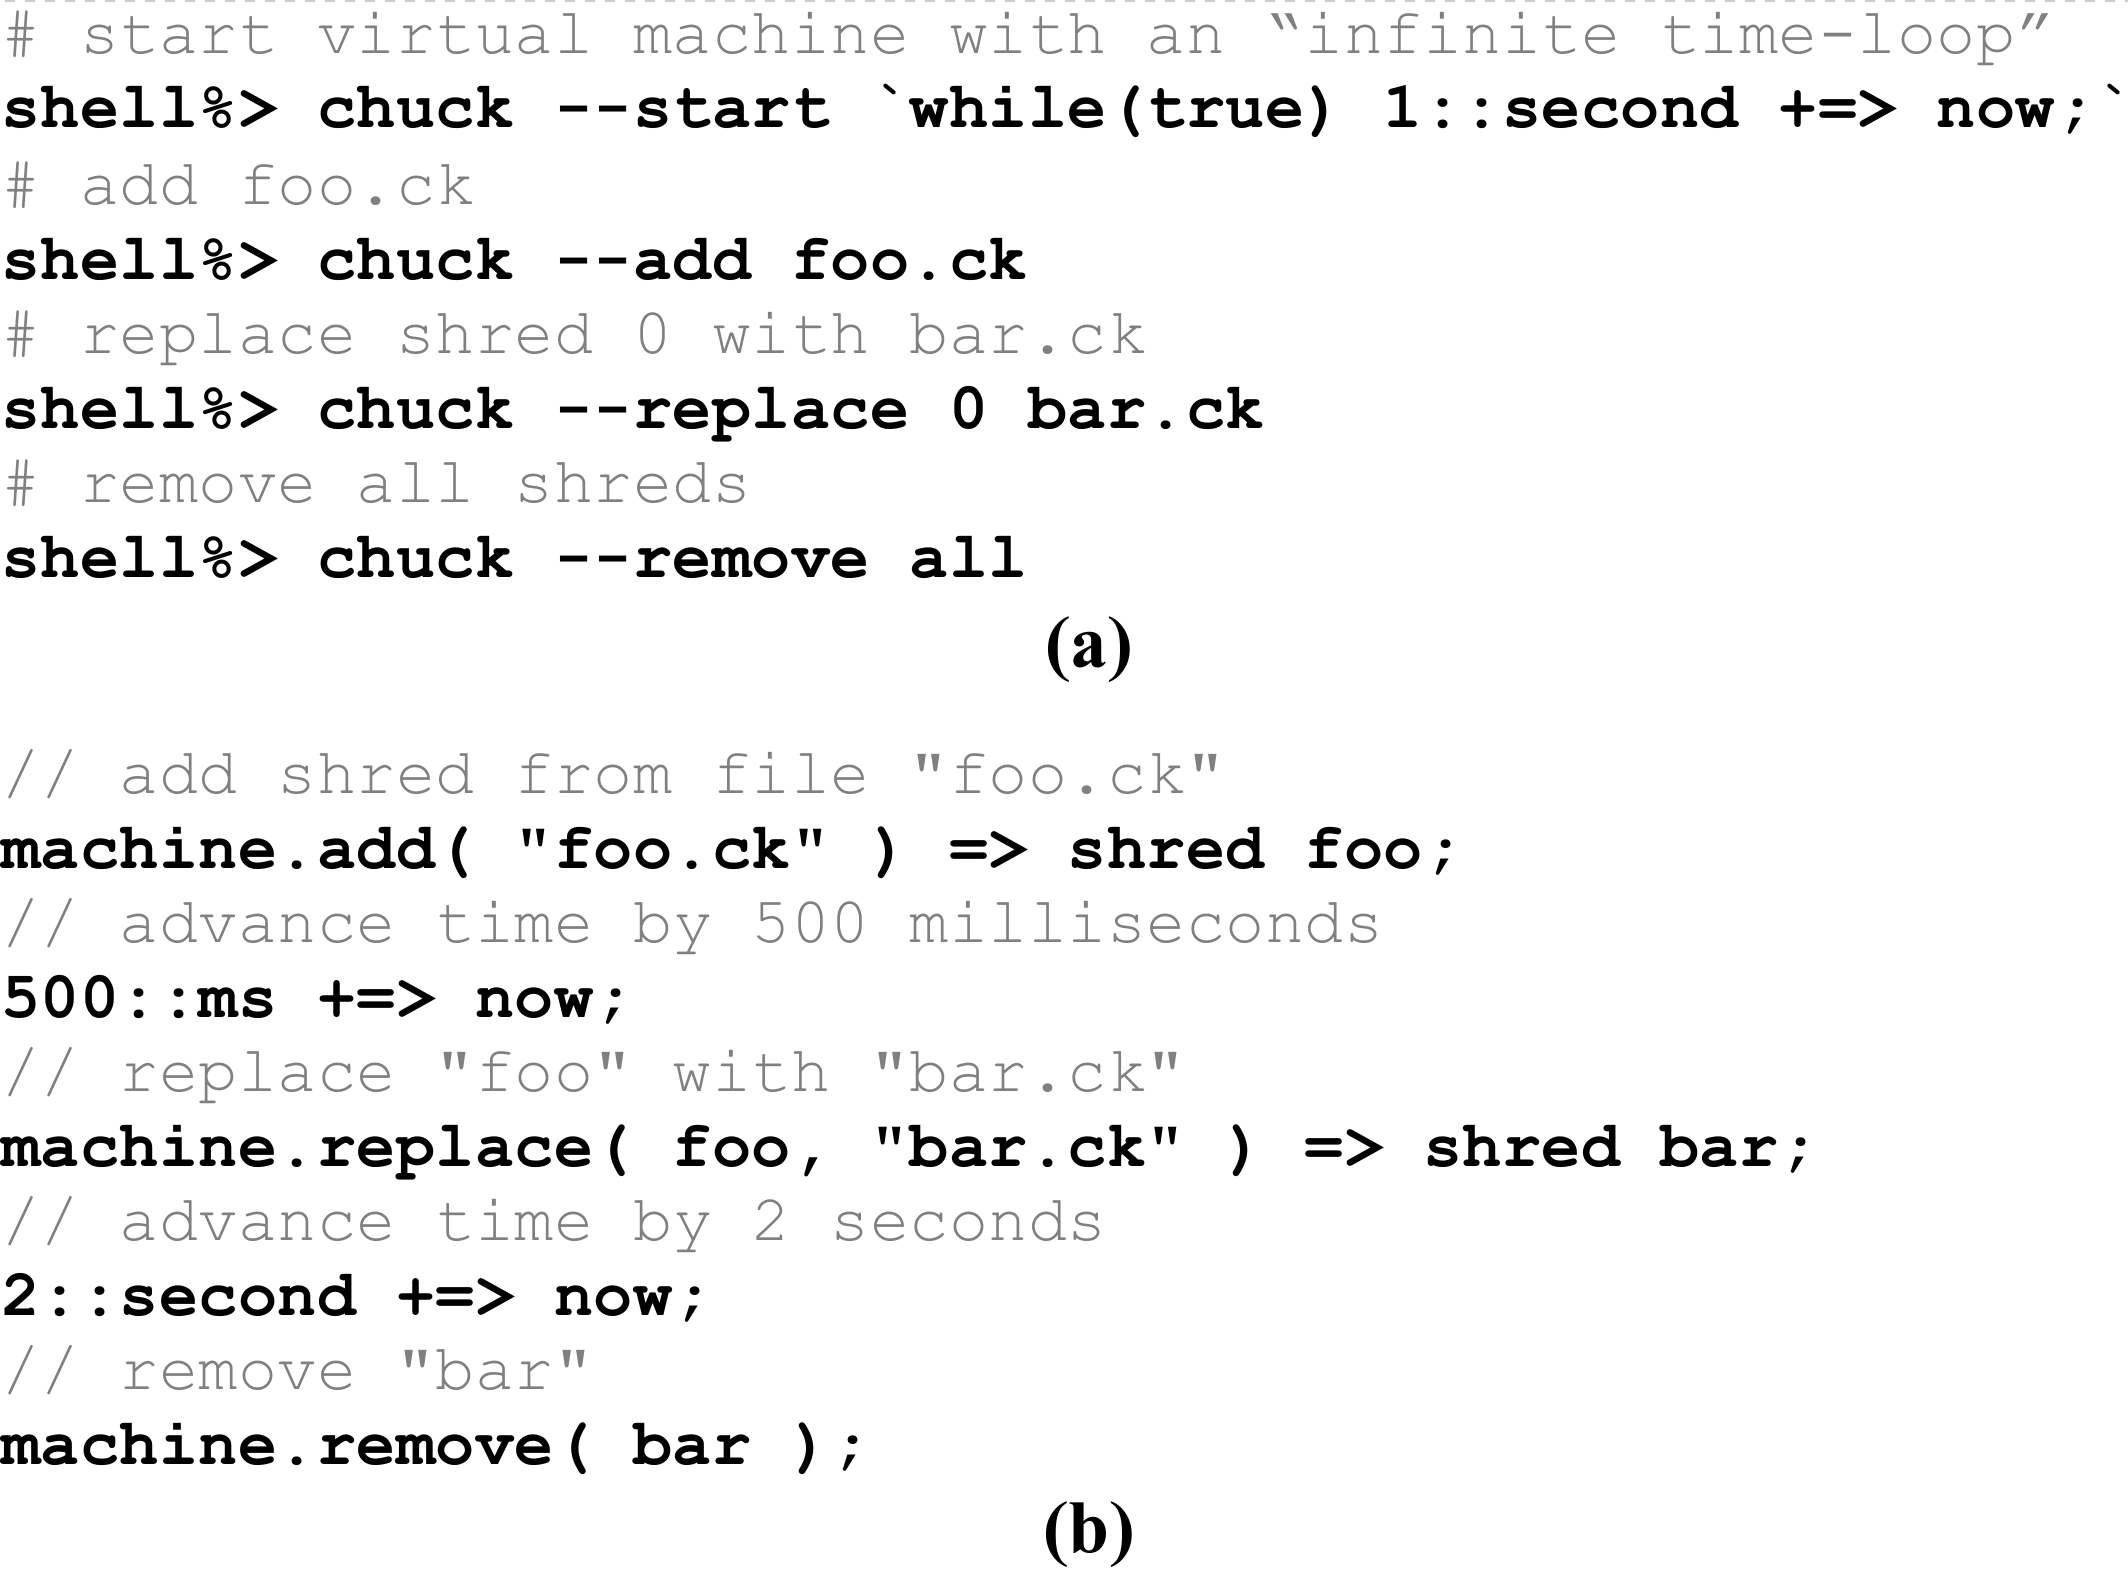
\includegraphics[width=90mm]{fig6.png}
\caption{Two examples of using the runtime code management interface:\textbf{ (a)} from a command-line shell, \textbf{(b)} from within a shred, which has timing control.}
\label{Wang:img-6}
\end{figure}

% Tried code, but better with figure

%\begin{verbatim}
%# (a)
%# start virtual machine with an “infinite time-loop”
%shell%> chuck --start `while(true) 1::second +=> now;`
%# add foo.ck
%shell%> chuck --add foo.ck
%# replace shred 0 with bar.ck
%shell%> chuck --replace 0 bar.ck
%# remove all shreds
%shell%> chuck --remove all%

%// (b)
%// add shred from file "foo.ck"
%machine.add( "foo.ck" ) => shred foo;
%// advance time by 500 milliseconds
%500::ms +=> now;
%// replace "foo" with "bar.ck"
%machine.replace( foo, "bar.ck" ) => shred bar;
%// advance time by 2 seconds
%2::second +=> now;
%// remove "bar"
%machine.remove( bar );
%\end{verbatim}



The ``code-runs-code'' feature is powerful because it allows a program to self-manage shreds on-the-fly with sample-synchronous precision.  Users can also assimilate shreds that systematically add (potentially many) additional shreds, each with precise timing.  Because the compiler and the virtual machine run in the same process, much of the intermediate processing can be eliminated. Finally, the ability to evaluate strings as code (currently unimplemented) at runtime would open the possibility for self-generating on-the-fly programs with fast compilation-to-runtime response.

The status feedback is helpful for quickly surveying the state of the system and is particularly useful in an \textit{on-the-fly} setting because it can identify hanging or non-cooperative shreds.   For example, if the system runs a shred containing an infinite loop, it will fail to yield and cause the virtual machine execution unit to hang indefinitely.  This type of behavior cannot be reliably detected at compile time, as the Halting Problem demonstrates.  However, the \textit{on-the-fly} programmer can identify and remove misbehaving shreds from the virtual machine \textit{manually}, resulting in minimal interruption to the performance or session.  While this recovery mechanism is far from perfect, it is far more advantageous than killing the system and restarting.  Additionally, it can help the composer/performer tune the system by identifying shreds that are taking too much CPU time and optimize them individually.

This high-level semantic uses concurrent shreds as modules and provide a means of managing them.  However, this interface alone is not adequate for specifying timing between incoming and existing modules.  This brings us to the internal timing semantic of the on-the-fly programming model.

\subsubsection{ Internal Semantics}

The internal semantics deal with the problem of precise timing between on-the-fly modules.  The goal is to provide a consistent and accurate mechanism for shreds to synchronize with each other.  In our model, the semantics are natural extensions of the ChucK timing mechanism.  By querying and manipulating time using the special variable \verb!now!, the programmer can determine the current time, and specify how the code should respond.

By the properties of ChucK timing and concurrency:  (1) \verb!now! always holds the current ChucK time, (2) changing the value of \verb!now! \textit{advances} time in ChucK and has the side effect of blocking the current shred (allowing audio and other shreds to compute) until \verb!now! holds the value that was assigned to it,  (3) if {\small t} is of type {\small time}, {\small t => \textbf{now}} advances time until {\small t }equals{\small  now}, (4) if {\small d} is of type {\small dur }(a duration), {\small d +=> \textbf{now}} advances time by {\small d}.  We illustrate this below with some common code segments that \textit{synchronize to time}.

\begin{itemize}
	\item Let time pass for some duration (in this case 10 seconds)
\end{itemize}

\begin{verbatim}
now + 10::second =¿ time later;
later =¿ now;
// or simply:
10::second +=¿ now;
\end{verbatim}


\begin{itemize}
	\item \textit{Synchronize} to some absolute time t
\end{itemize}

\begin{verbatim}
t => now;
\end{verbatim}


\begin{itemize}
	\item \textit{Synchronize} to absolute time t or later
\end{itemize}

\begin{verbatim}
if( t < now ) t => now;
\end{verbatim}


\begin{itemize}
	\item \textit{Synchronize} to the beginning of next period of duration T
\end{itemize}

\begin{verbatim}
120::ms => dur T;
// period to synchronize to
T – (now % T) +=> now; // advance time by remainder
\end{verbatim}


\begin{itemize}
	\item \textit{Synchronize} to the beginning of next period, plus offset D
\end{itemize}

\begin{verbatim}
T – (now % T) + D +=> now;
\end{verbatim}


\begin{itemize}
	\item Start as soon as possible
\end{itemize}

\begin{verbatim}
// no code necessary
\end{verbatim}


The semantic allows programmers to precisely specify many more timing and
synchronization behaviors.  These statements can be placed to impose timing at
arbitrary points in the program flow.  For the purpose of initial time-based
synchronizations in on-the-fly programming, they may be placed near the beginning
of a shred to synchronize to time before moving on.

\subsection{An On-the-fly Example}

Using the operational semantics described in Section 4.1, we construct a
simplified example: phasing on-the-fly.  We write three shreds, each to trigger
some sound at a slightly different rate, and we assimilate them one by one, with
time-based synchronizations specified for the second and third shreds.  The code
for the three shreds and the commands to add them are shown in Figure~\ref{Wang:img-7}.  (With
copy/paste, this can be realized in roughly 45 seconds.)


% \begin{verbatim}% 

% “a”=>sndbuf=>dac; 
% // first to run no need synch 
% while( true ){
%   // trigger snd
%   0 -> sndbuf.pos;
%   300::ms +=> now;
% }% 

% “b”=>sndbuf=>dac; 
% 300::ms => dur T;
% T–(now%T) +=>now; 
% while( true ){
%   // trigger snd
%   0 -> sndbuf.pos;
%   400::ms +=> now;
% }% 

% “c”=>sndbuf=>dac;
% 300::ms =>dur T;
% T – (now%T) +
% 150::ms +=> now;
% while( true ){
%   0 -> sndbuf.pos;
%   500::ms +=> now;
% }
% \end{verbatim}% 
% 

% \begin{verbatim}
% shell %> chuck --start left.ck
% shell %> chuck --add middle.ck
% shell %> chuck --add right.ck
% \end{verbatim}



\begin{figure}[t]
\centering
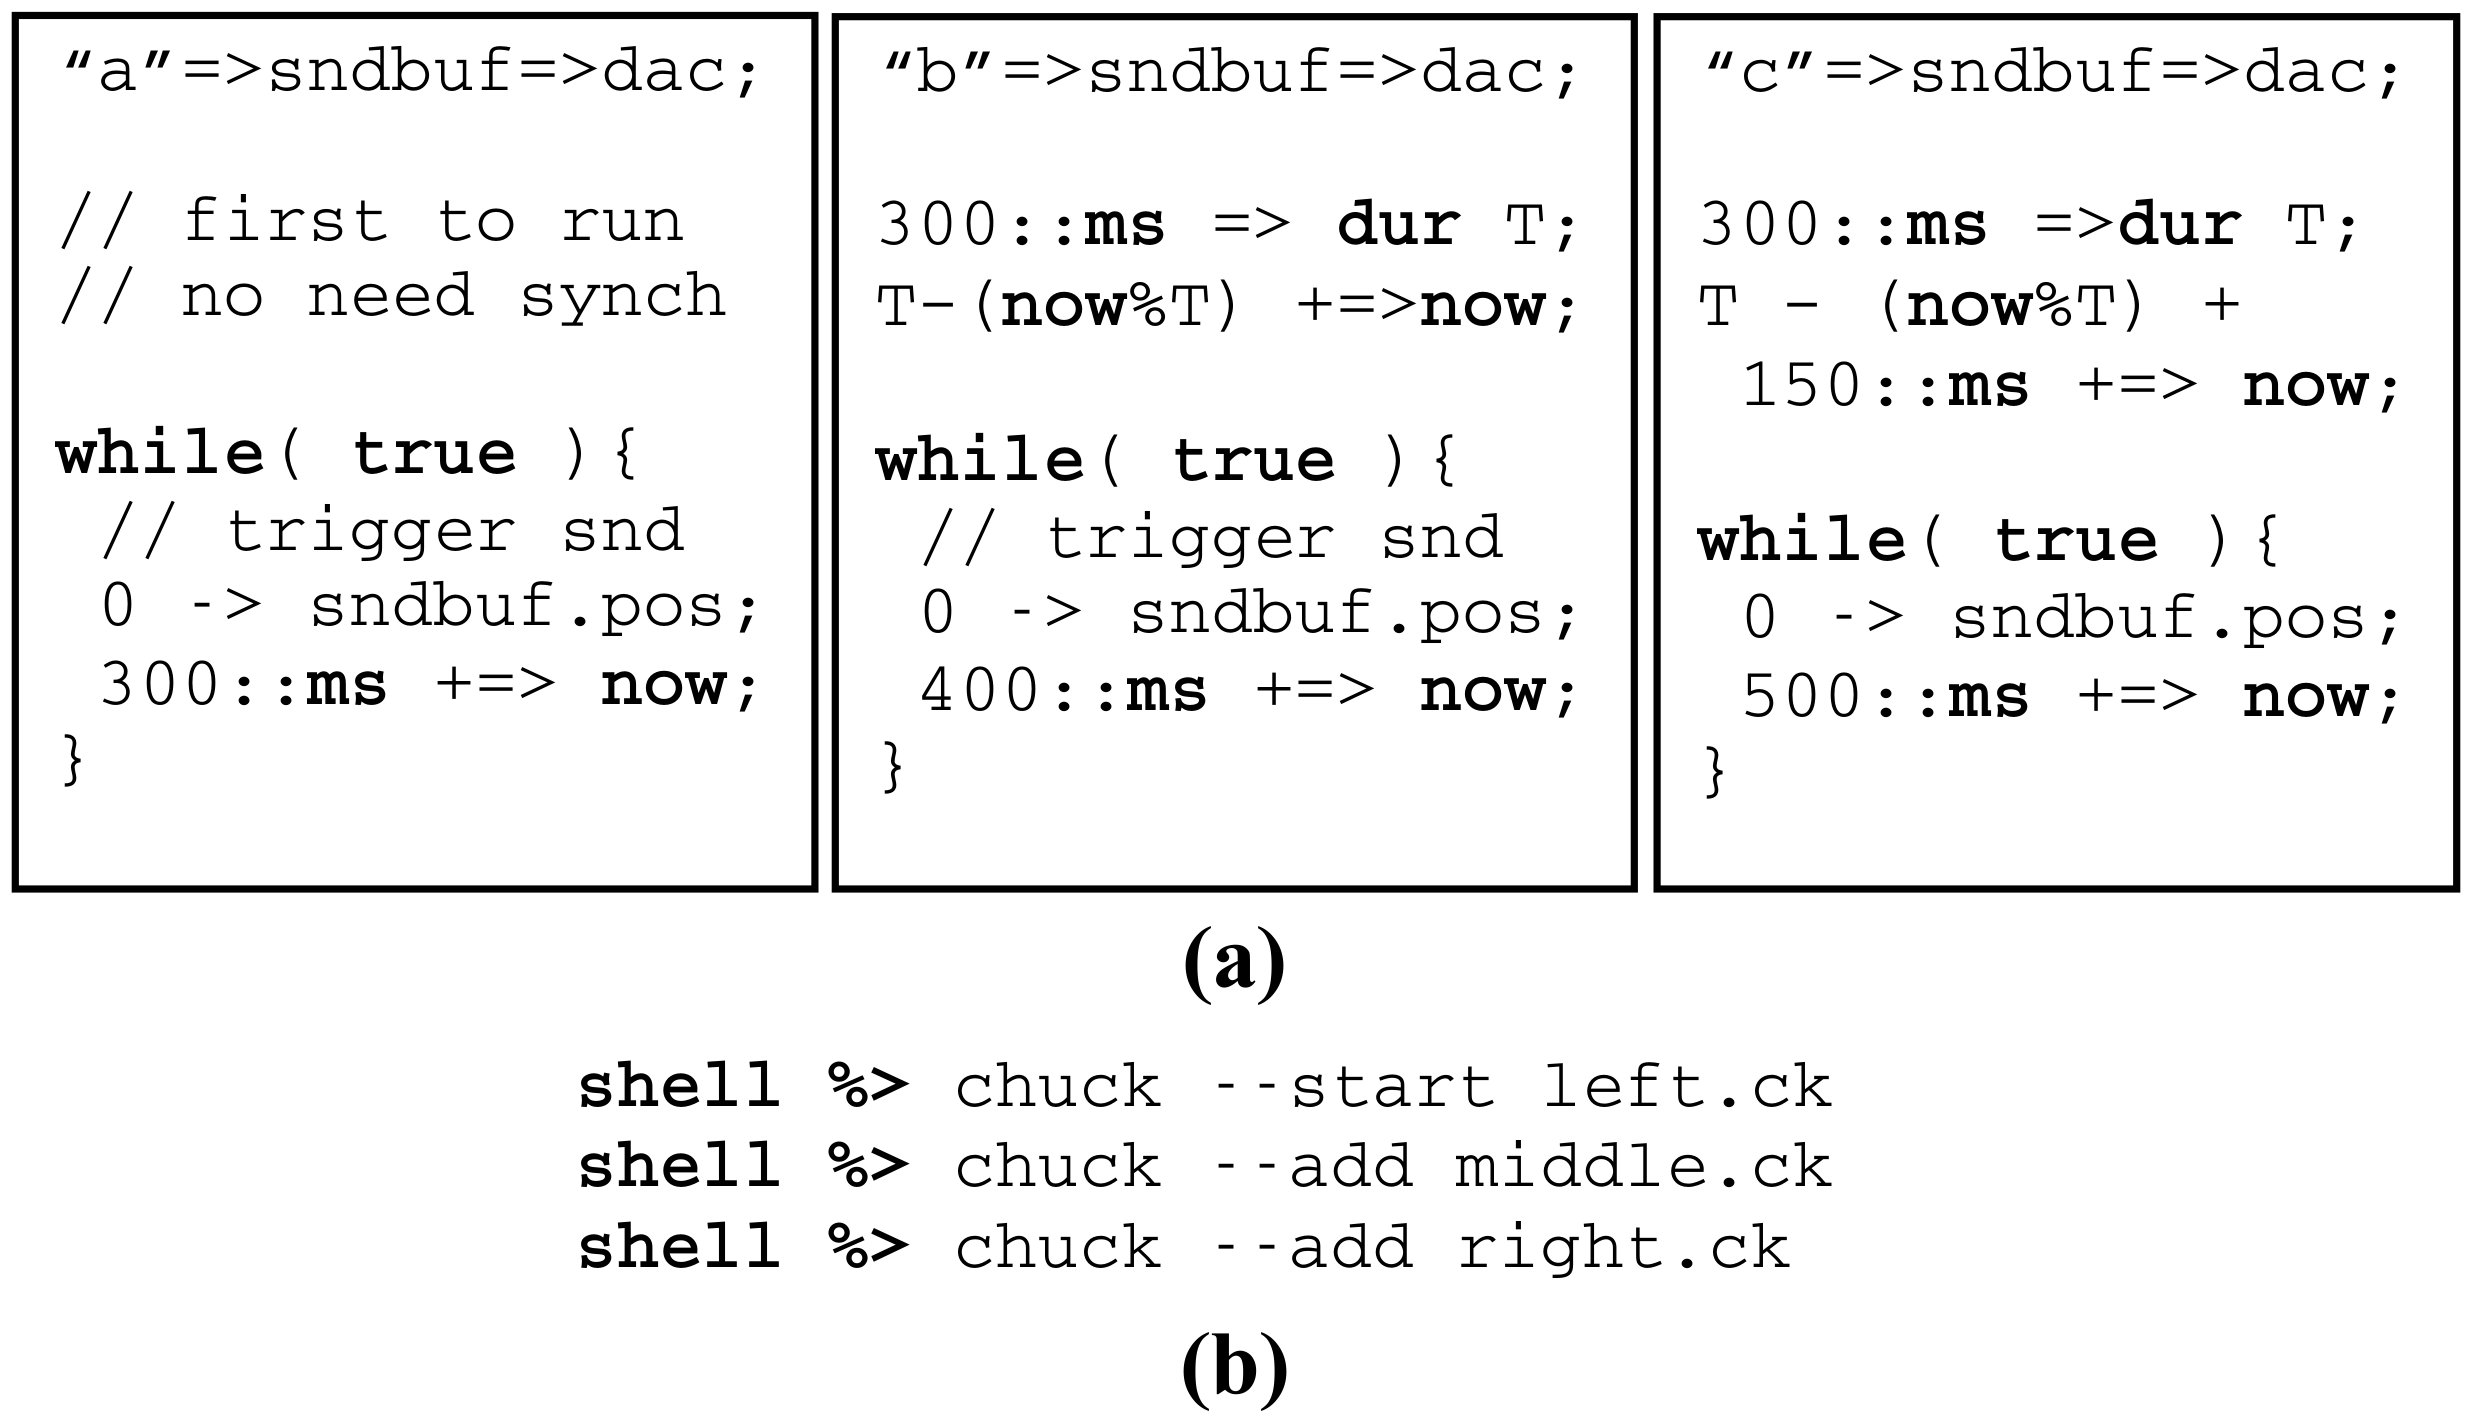
\includegraphics[width=240pt]{fig7.png}
\caption{(a) Code for three concurrent shreds, the middle shred synchronized to the cycle of the left shred, and the right shred synchronized to cycle of the left shred offset by 150 milliseconds. (b) Shell command to add them on-the-fly.}
\label{Wang:img-7}
\end{figure}



\subsection{Properties}

Recall the challenges we defined in \textit{Section 2.2}: modularity, timing,
conciseness, and flexibility.  Using the features of ChucK and the framework we
discussed, we briefly comment on the effectiveness of this model.

Concurrency provides a modular approach to breaking up the program into
manageable pieces that can be added, remove, and replaced, and also synchronized
to each other precisely, using the timing mechanism.  This framework preserves
the properties of timing in ChucK and extends them to an on-the-fly setting in an
attempt to unify high-level (musical), low-level (control rates), and
inter-modular (shred synchronization) timing into one system.  Finally, embedding
the timing specifications directly in the languages and using the ChucK operator
aims for cleaner and more maintainable code, which an on-the-fly programmable
system vitally demands.

\section{An Open On-the-fly Aesthetic}

Our on-the-fly aesthetic (Figure~\ref{Wang:img-8}) is one where the \textit{process of
on-the-fly programming} is conveyed to the audience.  It addresses two important
issues in computer music performance.  First, it can be argued that many
technical and aesthetic intentions are often difficult to discern in performance
where they do not have to be or should not be.   The on-the-fly programming
aesthetic can be seen as one approach to address this concern, for it provides a
channel for the audience to see both the intention and the results. 
Additionally, the appreciation of this aesthetic approach does not necessarily
hinge on the audience understanding the code (though this can certainly open new
dimensions); it is more fundamentally about the act (and art) of construction,
via coding.


\begin{figure}[t]
\centering
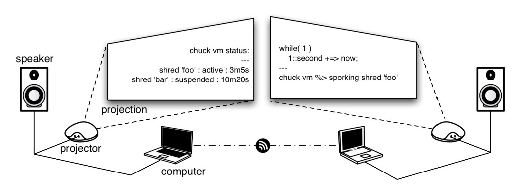
\includegraphics[width=\textwidth]{img-2-eps-converted-to-crop.pdf}
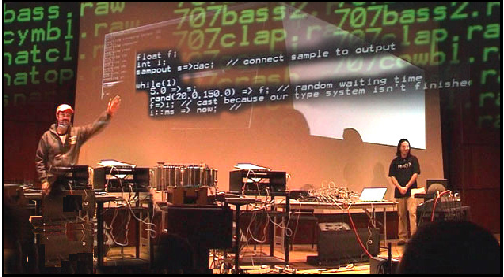
\includegraphics[width=\textwidth]{img-3-eps-converted-to-crop.pdf}
\caption{An on-the-fly performance for two laptops and two laptop
projectors. Note the two projections in the background.  Superimposed are two
projected screen shots from the performance. The schematic can be extended to any
number of performers.}
\label{Wang:img-8}
\end{figure}


The second topic that the on-the-fly aesthetic aims to address is that of
virtuosity in computer music.  On-the-fly programming supplies a platform where
the performer is able to render various types of mastery and creativity that can
be immediately appreciated, or at least perceived.  While typing speed may not
inspire, the general expressive power of programming languages opens unlimited
possibilities for clever approaches and beautiful design.  The timing semantic
facilitates ChucK code to be followed, aiding the audience to more readily
appreciate the design and construction of on-the-fly programs.

\section{Conclusions and Future Work}

We have outlined some central challenges in on-the-fly programming, and
presented a framework and an aesthetic for addressing them.  The ChucK virtual
machine provides a simple, yet powerful set of high-level operations to manage
shreds externally, and allows the program and incoming \textit{shreds} to manage
timing and synchronization internally in the code.  The concurrency model in
ChucK gives a natural boundary between on-the-fly modules of the program.  The
timing mechanism can be used in the same manner to synchronize the incoming code
to the rest of the program with single sample precision.  Additionally, the
syntax of the ChucK operator and the strong correspondence between timing and
program flow help to design and reason about code in a time-constrained,
on-the-fly setting.  In its entirety, this model yields a versatile tool to
create, manage, and further explore on-the-fly programs.

While this framework has many desirable properties, it still unpolished and
unwieldy in many respects, partly because coding inherently takes time.  Future
work may look into programming environments that understand the deep structure of
the program being written and facilitate writing and debugging on-the-fly.  The
performance aesthetic may explore visualizations of \textit{program}
\textit{state}---in addition to code.  Also, it would be interesting to
investigate reducing the modular granularity, allowing finer pieces of code to be
runtime modified.

\begin{acknowledgement}
We wish to sincerely thank Andrew Appel, Brian Kernighan, Ari Lazier, Nick
Collins and the authors of \cite{Collins:2003} for their support.  Also thanks to the anonymous
reviewers for their helpful comments.
\end{acknowledgement}


\section*{Author Commentary: Programming On-the-fly}

\paragraph{Ge Wang and Perry R. Cook}

This paper, written in early 2004, introduced the NIME audience to the formulation, aesthetic, and vision of on-the-fly programming/live coding---and through the lens of ChucK, a then fledgling computer music language and perhaps the first designed, at least in part, with live coding in mind.  This work helped to kickstart an era of live coding, exploring artistic goals of writing code as live performance, and the aesthetics that accompanied it (showing our screens in a new form of code-mediated insider art, the balance between software abstraction beforehand and manual manipulation of code during live performance, programming tool as musical instrument, etc.).  The impetus to explore on-the-fly programming arose from investigating laptop performance---and (of course) we weren't the only ones pondering and experimenting.  The works of Alex McLean (Hacking Perl in Nightclubs \cite{McLean:2004}), Nick Collins (who a few years later committed himself to a period of daily live coding practice, and wrote a NIME paper about the experience \cite{Collins:2007}), Julian Rohrhuber (responsible for SuperCollider's JITLIB), Dave Griffith (live coding graphics via Fluxus) and a handful of others also influenced and contributed to the emergence of a new community.

All of this helped to spawn TOPLAP (whose acronym sometimes expands to ``Temporary Organisation for the Pragmatics of Live Art Programming'' and whose motto has been ``Taking the routine out of subroutine since 2004;'' the organization even released a CD in 2007 \cite{TOPLAP:2007}), and to raise awareness of live coding as a practice, ethos, and mindset of working with sound, visuals, interaction.  Since that time (and despite the ``Temporary'' in TOPLAP---which I think was us being realistic about its prospects and longevity back in 2004), live coding has become a sustained, stable practice and discipline, and environments for on-the-fly programming proliferated with the likes of Impromptu (which gave rise to Extempore), Sonic Pi, Gibber, Tidal, Overtone, UrMus, EarSketch, \ldots the list goes on.\footnote{\url{http://toplap.org/category/software}}  These environments explore live art programming in a variety of contexts, spanning web browsers, mobile devices, circuit bending, virtual reality, and more---going well beyond the laptop performance paradigms that originally precipitated it.

As for the formulation of on-the-fly programming in ChucK (and as related to its properties of temporal determinism and sample-synchronous concurrency), much has transpired and evolved.  This paper envisioned ``programming environments that understand the deep structure of the program being written and that facilitate writing and debugging on-the-fly,'' which became the live analytics-driven, graphically intensive, and ultimately ill-fated Audicle.  Fortunately, this eventually led to Spencer Salazar's miniAudicle in 2006, which has since become the predominant integrated development environment for the ChucK world, and where the primary vestiges of the original on-the-fly programming system now reside.  Applications of on-the-fly programming and ChucK can be found in various settings---teaching, demonstration, and experimentation in the classroom (it has become a natural way to teach computer music in face-to-face courses at Princeton, Stanford, and CalArts, as well as in massively open online courses on Kadenze and Coursera), sound design labs, digital workbenches for new instruments and more.  On-the-fly programming engenders a rapid experimentation mindset that has greatly benefited the prototyping of new instruments in laptop orchestras (PLOrk, SLOrk, the Machine Orchestra), even when the majority of finished musical works are not live coded.  The early mobile apps of Smule like Ocarina \cite{Wang:2014} not only uses ChucK as the sound engine, but have also benefited from its rapid prototyping of both sound and interaction.  The original tenets of strong-timing in ChucK, more than 10 years later, continue to give on-the-fly programming in ChucK its own distinctive nuances \cite{Wang:2015}.

Over the course of the decade since the original paper, the computer world has evolved in profound ways (mobile, wearable, social, augmented, virtual), and the exploration of ``in-the-moment'' programmability has organically evolve alongside it.  The sophistication of tools and the ways of thinking they foster have come a long way (in not a long time) since the time of this paper---improving, refining, and redefining the early approaches in on-the-fly programming.  Yet the original ethos---of exploring the agency and mindset of live programming as creative gestures---remains alive and vibrant.  It has been an interesting and unexpected journey, and one that continues.



\section*{Expert Commentary: Coding as Musical Performance}

\paragraph{Georg Essl}

One of the hallmarks of a vibrant field of inquiry is its persistent need to revisit its most fundamental definitions. One such defining question is this: ``What is an interface for musical expression?'' Certainly, the canonical view of a musical instrument is a technological artifact designed for musical performances, usually in a mode where musical gestures lead to musical sounds. However, with ``live coding,'' interactions that were originally neither performative nor musical can be re-envisioned as such. In doing so, they expand our notion of what musical interfaces are! Making this very insight explicit is perhaps the most significant claim to fame of Wang and Cook's 2004 NIME paper.

Laptops had already been a performance platform for a while when suddenly, in the early years of the twenty-first century, the idea emerged that writing musical computer programs live on stage could be an exciting performance practice.  Early pioneers drew on existing systems to realize the performance practice \cite{Collins:2003}.

The work of Ge Wang and Perry Cook stuck out in that environments were built from scratch that were meant to directly support this new kind of performance art. The field was just emerging and what Wang and Cook called ``on-the-fly'' would later be subsumed under the term ``live coding.'' 

The centerpiece of the contribution was the design of the programming language ChucK, which later was also supported by efforts in programming environment design. There are many innovations surrounding the programming language ChucK and the systems that support it. But in the context of the 2004 NIME paper, the central contribution is that it advocates taking a programming language as part of a performance interface seriously.

The key question here remains ``what should a programming language look like, if it is understood to be part of a performance interface?.'' Programming languages have multiple layers in which they operate with respect to their use and function. A lower layer is its functionality. Wang and Cook realized that time plays a very important role in music performance. Hence, ChucK introduces first principle time primitives in its programming functionality. Higher level layers are associated with choices in syntax and semantics of the language. In the synthesis environment, audio dataflow is a critical element. ChucK introduces the ascii-graphical ChucK-operator (\verb!=>!) that represents this connectivity and data flow. It further also serves to provide assignments and can be used to advance time programmatially.

The mix of new operators and types with well established C-style language syntax made ChucK a modern, yet surpisingly accessible, sound synthesis programming language well-suited for emerging live coding.

The design of live coding environments and languages has remained a vibrant and important research area \cite{Roberts:2014}  and can transcend textual representations \cite{McLean:2010}. Evidence points to the possibility of different good representations for different user types and scenarios \cite{Eaglestone:2007}. In this light, we can view Wang and Cook as a proposal to an answer within the context of a persistent yet deeply important open research question.

Live coding has in the last decade developed as a rich and complex field, being nurtured by symposia, workshops, and conferences solely dedicated to the topic. Yet, its scope is still expanding.

Live coding is a kind of writing activity specifically confined to the content of the writing. Recently, Sang Won Lee has proposed a generalization of this idea \cite{Lee:2015}: What if we conceive of any act of writing as potentially performantive? Live coding then becomes a special case of live writing where the written content is confined by the syntactic, semantic, functional, and performative context of live programming. This is particularly interesting in the emerging trend of collaborative live coding, where multiple programmers work jointly on a performance. This helps study more clearly what aspect of collaboration is particular to collaborative programming and what aspects are generic to any joint writing task.

Live-coding today does look very different than it did when Wang and Cook published their paper at NIME 2004. Presently it includes new research questions such as: How to facilitate long-distance networked collaboration? How does a crowd-sourcing paradigm fit into live performance? How can prediction and machine learning fruitfully be included to achieve even more liveness? In hindsight, the Wang and Cook paper stands as one of the early seminal papers of a topic that developed into its own field of inquiry.

